%KELOMPOK 4 Blank-On1
%\begin{enumerate}
%\item Andri Fajar Sunandhar
%\item Cokro Edi Prawiro
%\item Fadila
%\item Sandro Samuel Sinaga
%\end{enumerate}



\section{Common Gateway Interface}
CGI merupakan metode yang dipakai untuk mempertukarkan data di antara server dan klien (browser). CGI merupakan sebuah standar dimana program atau script bisa mengirim data kembali ke web server dimana ia diproses, yaitu dengan menggunakan tag HTML standar untuk mendapatkan data dari seseorang, kemudian meneruskannya ke CGI. Selanjutnya CGI melakukan serangkaian aksi terkait data tersebut\cite{prihatmoko2013pengembangan}.



\par CGI adalah interface untuk menjalankan program-program eksternal,dibawah informasi server, biasanya server HTTP (walaupun CGI standar dirancang untuk lintasan-platform yang
menangani semua jenis hardware dan software yang berbeda, windows CGI 1.3 khusus untuk platform microsoft Windows 95/98 dan windows NT). Dengan CGI server bisa
melayani informasi yang tidak ada dalam format yang mudah dibaca oleh client,seperti data yang ada dalam database SQL, dan melakukan gateway antara dua sesuatu yang 
dihasilkan oleh browser client. Seringkali program gateway ini disebut script.

\par Sebuah server web memproses permintaan klien CGI menggunakan skrip atau aplikasi CGI. Sebagai contoh, ketika sebuah database ditanyakan oleh klien, 
server web bertindak sebagai gateway antara database dan klien. Server web mentransmisikan permintaan klien ke aplikasi CGI yang melakukan kueri basis data,
 memformat hasil dan mengembalikan data berformat HTML ke server web. Server web kemudian mentransmisikan data berformat HTML ke klien untuk ditampilkan kepada pengguna.




\par Adapun pengertian lain dari Common Gateway Interface yaitu sekumpulan aturan untuk mengarahkan sebuah server web berkomunikasi dengan software dalam mesin yang sama begitu pula sebaliknya antara software CGI programs dengan web server. Setiap perangkat lunak dapat menjadi perogram CGI dengan syarat software tersebut dapat melakukan input dan output sesuai setandar CGI. CGI menjadi setandar menghubungkan untuk menghubungkan data informasi yang terjadi antara server dan aplikasi, seperti HTTP. Script CGI dapat mengirtimkan data kembali ke web server  dimana CGI diperoses. CGI merupakan interface antara halaman website dengan web server yang menjalankan perogram\cite{aditya2015analisis}.

\begin{figure}[ht]
\centerline{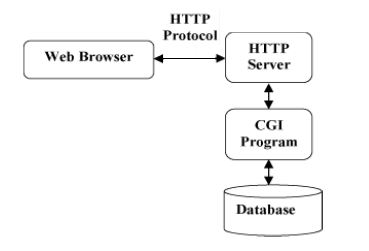
\includegraphics[width=1\textwidth]{figures/1arsitekturCGI.JPG}}

\caption{CGI Arsitektur Diagram} 
\label{1arsitekturCGI}
\end{figure}

Gambar\ref{1arsitekturCGI} menjelaskan bahwa antara HTTP server di pelantarai oleh CGI program dalam mengakses data 
dari database. Jadi jika data yang diminta di batasi atau tidak memiliki hak akses oleh CGI data tersebut tidak dapat di munculkan 
oleh web browser.  Cara untuk memahami perinsip dari (Common Gateway Interface ) CGI, dapat dicoba dengan melakukan click pada suatu URL suatu website.
setelah melakukan hal tersebut browser akan menghubungi HTTP web server dan meminta URL dari website tersebut. Kemudian web server tersebut akan
mengurai (prasing) URL dan akan mencari berkas dari link tersebut, bila ditemukan maka akan diteruskan ke browse, begitu juga sebaliknya jika tidak ada
maka akan diberikan pesan error. lalu web browser akan menampilkan hasilnya, baik url yang tadi diminta maupun pesan error karena URL yang dituju tidak ada. Meski begitu, ada kemungkinan untuk mengatur suatu HTTP server untuk membatasi akses terhadap suatu berkas.
jadi halaman URL yang dituju tidak bisa diakses hal tersebut merupakan fungsi dari CGI script. supaya lebih paham dapat dilihat 
pada arsitektir program CGI.



\par Salah satu kekuatan utama yang memungkinkan developer web membangun aplikasi-aplikasi web yang dinamis adalah kemampuan server web untuk mengakses sistem database. Untuk keperluan pengembangan aplikasi web yang dinamis, pertama kali diperkenalkan Common Gateway Interface (CGI). CGI adalah bagian dari server web yang dapat berkomunikasi dengan program lain di luar server web. CGI memungkinkan server web memanggil suatu program, lalu mengirimkan data-data spesifik dari pengguna ke program tersebut. Hasil proses tadi diterima oleh CGI yang selanjutnya menyerahkannya kepada server web untuk kemudian, yang pada gilirannya akan mengirimkan informasi tersebut kembali dalam bentuk HTML ke browser web pengguna\cite{ibrahim2011sistem}.

\section{PHP and Common Gateway Interface interconnections }
Common Gateway Interface is a standard that is used to connect various application programs to web pages. One example of the programming language is PHP. PHP is a software that is open source and can pass across the various platform. Php can be run in 2 ways ie as apache module in web server and also as binary in Common Gateway Interface.This language was created in 1994 by Ramus Lerdoff.  Initially, PHP is a CGI program that is devoted to receiving input through forms displayed in web pages or browser. The PHP code is usually processed by a PHP interpreter which is usually executed as a native web server module or Common Gateway Interface\cite{nahado2015bumbu}.


\section{Security in Common Gateway Interface }
Common Gateway Interface is used to connect WWW (World Wide Web) systems with software or other software on the web server. The presence of the Common Gateway Interface allows connection interactive between the user and also the web server. Common Gateway Interface itself is often used as a mechanism to get information from users through "fill out a form", access the database, or generate dynamic pages. Although in principle the mechanisms in the Common Gateway Interface do not have security holes, programs or scripts created as CGI can have security flaws either created intentionally or unintentionally. That is because CGI program itself is run on the web server to use the web server resources.


\section{The Application of Common Gateway Interface }
CGI is applied to the making of applications involving python language with PHP language. CGI itself is implemented or modified as CGI Fast CGI protocol, where its function in the application is as an interface in other applications to the web server which is an alternative facility to improve its own performance for CGI which is intended for the web server application process which is Apache web server to dynamic language another. Processes and handling from CGI to FastCGI can be demonstrated from the use of this working support facility such as python as the dynamic language used and the fastCGI module for the server to be used on RFC2109 proxy caching.